\section{\normalsize POSSÍVEIS RESOLUÇÕES DO PROBLEMA}
	Primeiramente é importante frisar que existem diversas soluções para esse problema, algumas utilizando \textit{mutex}, outras utilizam semáforos, outros ainda utilizam os dois. Fora isso, existem soluções que compartilham o dado e promovem a concorrência através da criação de \textit{threads} enquanto outros soluções utilizam processos separados acessando uma memória compartilhada ou um arquivo para tal.
	
	Dito isso, e visando manter uma maior coerência deste relatório para com o leitor, não haverá um aprofundamento em todas as possíveis soluções para esse problema, ao invés disso, haverá uma explicação de qual deve ser a lógica utilizada pelo desenvolvedor para obter a melhor solução. Para tal, serão apresentadas duas soluções, melhor ao longo deste relatório.
	
	As políticas seguidas no caso dos leitores e escritores para acesso a região critica são as seguintes: 
	\begin{itemize}
		\item processos ou \textit{threads} leitores somente leem o valor da variável compartilhada (não alteram o valor da variável compartilhada), podendo ser de forma concorrente; 
		
		\item processos ou \textit{threads} escritores podem modificar o valor da variável compartilhada, para isso necessita de exclusão mutua sobre a variável compartilhada; 
		
		\item durante escrita do valor da variável compartilhada a operação deve ser restrita a um único escritor; 
		
		\item para a operação de escrita não se pode existir nenhuma leitura ocorrendo, ou seja, nenhum leitor pode estar com a região critica bloqueada; 
		
		\item em caso de escrita acontecendo, nenhum leitor conseguirá ter acesso ao valor da variável.

	\end{itemize}		
	
	\begin{comment}
	Continuando a análise do banco de dados e seguindo as políticas dos leitores e escritores têm as seguintes situações: 
	\begin{itemize}
		\item vários usuários consultando a tabela Estoque sem alterá-la; 
		\item para um usuário atualizar uma venda é necessário que não se tenha nenhum usuário consultando a tabela de estoque; 
		\item quando um usuário estiver atualizando a venda, nenhum outro usuário pode atualizar ao mesmo tempo; 
		\item se o usuário iniciar uma consulta e estiver ocorrendo uma atualização o mesmo irá esperar a liberação da atualização.
	\end{itemize}		
	\end{comment}
	
	Uma das soluções para esse problema, que se encontra no arquivo \textbf{first.c}, consiste na adição de garantias de acesso à região crítica pelos processos ou \textit{threads}. Para obter o acesso à base de dados, o primeiro leitor faz um \textit{down} no semáforo \textit{db}. Os leitores subsequentes meramente incrementam um contador, \textit{rc}. Conforme saem, os leitores decrescem o contador em uma unidade e o último leitor a sair faz um \textit{up} no semáforo, permitindo que um eventual escritor bloqueado entre.
	
	De forma simplificada o funcionamento dessa solução pode ser interpretado da seguinte forma:
	\begin{lstlisting}[style=C]
sem_t mutex;	/* controla o acesso a 'rc', que será usada posteriormente para verificar se existem leitores na seção crítica */
sem_t db;	/* controla o acesso a base de dados. Neste caso se trata de um acesso direto na memória, mas poderia ser um acesso à um arquivo ou banco de dados */
int rc = 0;	/* número de processos lendo ou querendo ler */
	\end{lstlisting}
	

\begin{minipage}[t]{0.45\linewidth}
\begin{lstlisting}[style=C]
void reader(void) {
  while(TRUE) { // repete para sempre
    down(&mutex); // obtém acesso exclusivo a região critica
    rc = rc + 1; // um leitor a mais agora
    if (rc == 1) 
    	down(&db); //se este for o primeiro leitor bloqueia a base de dados

    up(&mutex) // libera o acesso a região critica

    read_data_base(); //acesso aos dados

    down(&mutex); // obtém acesso exclusivo a região critica
    rc = rc -1; // menos um leitor
    if (rc == 0) 
    	up(&db); // se este for o último leitor libera a base de dados

    up(&mutex) // libera o acesso a região critica
  }
}
\end{lstlisting}
\end{minipage}
%
\begin{minipage}[t]{0.45\linewidth}
\begin{lstlisting}[style=C]
void writer(void) {
	while (TRUE) { // repete para sempre
	down(&db); // obtém acesso exclusivo
	write_data_base(); // atualiza os dados
	up(&db); // libera o acesso exclusivo
	}
}
\end{lstlisting}
\end{minipage}

	Tal solução, apesar de evitar a espera ocupada\footnote{que é um dos maiores problemas de comunicação entre processos ou \textit{threads}} e ter um bom desempenho, contém um problema sutil que vale a pena ser comentado. Suponha que, enquanto um leitor está usando a base de dados, um outro leitor chegue. Como ter dois leitores ao mesmo tempo não é um problema, o segundo leitor é admitido. Um terceiro leitor e outros subsequentes podem também ser admitidos se chegarem.
	
	Agora, imagine que chegue um escritor. O escritor não pode ser admitido na base de dados, pois escritores devem ter acesso exclusivo. O escritor é então suspenso. Leitores adicionais chegam. Enquanto houver pelo menos um leitor ativo, leitores subsequentes serão admitidos. Como consequência dessa estratégia, enquanto houver um fluxo estável de leitores chegando, todos entrarão assim que chegarem. O escritor permanecerá suspenso até que nenhum leitor esteja presente. Se um novo leitor chegar - supondo a cada dois segundos - e cada leitor levar cinco segundos para fazer seu trabalho, o escritor nunca entrará, sofrendo, então, de \textit{livelock} ou \textit{starvation}.
	
	O programa poderia ser escrito de um modo um pouco diferente: se um leitor chegar quando um escritor estiver esperando, o leitor será suspenso logo depois do escritor, em vez de ser admitido de imediato. Essa solução, assim como as soluções do problema convencional, possuem diversas formas de ser implementada, como, por exemplo, ao usar um \textit{mutex} que garante que o escritor poderá acessar a zona crítica, ou com uma variável global que indica se um escritor está querendo entrar na zona crítica. Independente de como a solução seja implementada, o escritor, para entrar na zona crítica, precisa esperar apenas pelos leitores que estavam ativos quando ele chegou, mas não por leitores que chegaram depois dele. A desvantagem dessa solução é que se consegue menos concorrência e, portanto, um desempenho menor. Tal solução está presente no arquivo \textbf{second.c}.
	
	No demais, segue, em anexo, uma Rede de Petri que apresenta uma solução genérica para o problema.
	
	\begin{figure}[H]
		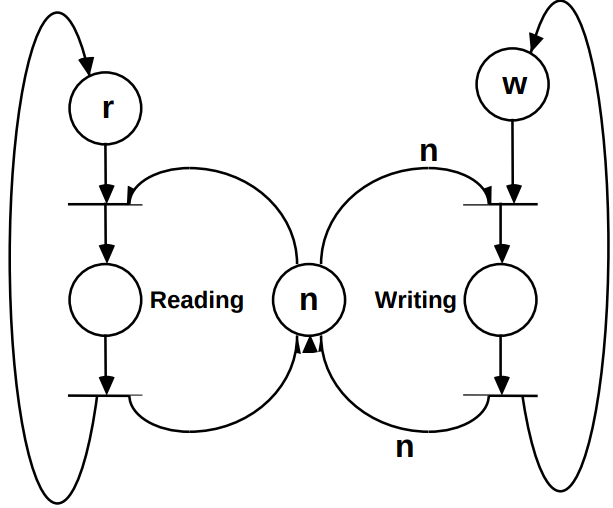
\includegraphics[scale=.7]{pictures/picture_01}
	\end{figure}